% Format teze zasnovan je na paketu memoir
% http://tug.ctan.org/macros/latex/contrib/memoir/memman.pdf ili
% http://texdoc.net/texmf-dist/doc/latex/memoir/memman.pdf
% 
% Prilikom zadavanja klase memoir, navedenim opcijama se podešava 
% veličina slova (12pt) i jednostrano štampanje (oneside).
% Ove parametre možete menjati samo ako pravite nezvanične verzije
% doktorata za privatnu upotrebu (na primer, u b5 varijanti ima smisla 
% smanjiti 
\documentclass[12pt,oneside]{memoir}

% Paket koji definiše sve specifičnosti doktorata Matematičkog fakulteta
\usepackage{matfdoktorat}
%
% Podrazumevano pismo je ćirilica.
%   Ako koristite pdflatex, a ne xelatex, sav latinički tekst na srpskom jeziku
%   treba biti okružen sa \lat{...} ili \begin{latinica}...\end{latinica}.
%   Tekst na engleskom jeziku okružiti sa \begin{english}...\end{english}.
%
% Opcija [latinica]:
%   ako želite da pišete latiniciom, dodajte opciju "latinica" tj.
%   prethodni paket uključite pomoću: \usepackage[latinica]{matfdoktorat}.
%   Ako koristite pdflatex, a ne xelatex, sav ćirilički tekst treba biti
%   okružen sa \cir{...} ili \begin{cirilica}...\end{cirilica}.
%
% Opcija [cirlat]:
%   ako se koristi xelatex, ovom opcijom uključujete mogućnost da tekst na 
%   srpskom jeziku unosite latinicom, a da se on prikazuje ćirilicom. U tom 
%   slučaju tekst koji želite da ostane latinicom morate okružiti sa
%   \lat{...} ili 
%   \begin{latinica}...\end{latinica}.
%   Tekst na engleskom jeziku okružiti sa \begin{english}...\end{english}.
%
% Opcija [biblatex]:
%   ako želite da koristite reference na više jezika i umesto paketa
%   bibtex da koristite BibLaTeX/Biber, dodajte opciju "biblatex" tj.
%   prethodni paket uključite pomoću: \usepackage[biblatex]{matfdoktorat}
%
% Opcija [b5paper]:
%   ako želite da napravite verziju teze u manjem (b5) formatu, navedite
%   opciju "b5paper", tj. prethodni paket uključite pomoću: 
%   \usepackage[b5paper]{matfdoktorat}. Tada ima smisla razmisliti o promeni
%   veličine slova (izmenom opcije 12pt na 11pt u \documentclass{memoir}).
%
% Naravno, opcije je moguće kombinovati.
% Npr. \usepackage[b5paper,biblatex]{matfdoktorat}

% Pomoćni paket koji generiše nasumičan tekst u kojem se javljaju sva slova
% azbuke (nema potrebe koristiti ovo u pravim disertacijama)
\usepackage{pangrami}

% Paket koji obezbeđuje ispravni prikaz ćiriličkih italik slova kada
% se koristi pdflatex. Zakomentarisati ako na sistemu koji koristite ovaj
% paket nije dostupan ili ako ne radi ispravno.
\usepackage{cmsrb}

% Ostali paketi koji se koriste u dokumentu
\usepackage{listings} % listing programskog koda

% Datoteka sa literaturom u BibTex tj. BibLaTeX/Biber formatu
\bib{matfdoktorat-primer}

% Ime doktoranda na srpskom jeziku (u odabranom pismu)
\autor{Петар П. Петровић}
% Ime doktoranda na engleskom jeziku
\author{Petar P. Petrović}
% Naslov teze na srpskom jeziku (u odabranom pismu)
\naslov{Докторат из математике или рачунарства чији је наслов јако дугачак}
% Naslov teze na engleskom jeziku
\title{Doctoral Dissertation in Mathematics or Computer Science}
% Godina u kojoj je teza predana komisiji
\godina{2015}
% Ime i afilijacija mentora (u odabranom pismu)
\mentor{др Мика \textsc{Микић}, редовни професор\\ Универзитет у Београду, Математички факултет}
% Ime i afilijacija prvog člana komisije (u odabranom pismu)
\komisijaA{др Мика \textsc{Микић}, редовни професор\\ Универзитет у Београду, Математички факултет}
% Ime i afilijacija prvog člana komisije (u odabranom pismu)
\komisijaB{др Ана \textsc{Анић}, ванредни професор\\ University of Disneyland, Недођија}
% Ime i afilijacija drugog člana komisije (u odabranom pismu)
\komisijaC{др Лаза \textsc{Лазић}, доцент\\ Универзитет у Београду, Математички факултет}
% Ime i afilijacija četvrtog člana komisije (opciono)
% \komisijaD{}
% Datum odbrane (obrisati ili iskomentarisati narednu liniju ako datum odbrane nije poznat)
\datumodbrane{15.~јануар 2016.}

% Apstrakt na srpskom jeziku (u odabranom pismu)
\apstr{%
\pangrami
}

% Apstrakt na engleskom jeziku
\abstr{%
\pangrami

\pangrami
}

% Ključne reči na srpskom jeziku (u odabranom pismu)
\kljucnereci{анализа, геометрија, алгебра, логика, рачунарство, астрономија}

% Ključne reči na engleskom jeziku
\keywords{analysis, geometry, algebra, logic, computer science, astronomy}

% Šira i uža oblast teze na srpskom jeziku (u odabranom pismu)
\oblast{рачунарство}
\uzaoblast{биоинформатика}

% Šira i uža oblast teze na engleskom jeziku
\area{computer science}
\subarea{bioinformatics}

% Univerzalna decimalna klasifikacija (UDK tj. UDC)
% https://en.wikipedia.org/wiki/Universal_Decimal_Classification
\udk{004.415.5(043.3)}

\begin{document}
% ==============================================================================
% Uvodni deo teze
\frontmatter
% ==============================================================================
% Naslovna strana
\naslovna
% Naslovna strana na engleskom jeziku
\naslovnaen
% Strana sa podacima o mentoru i članovima komisije
\komisija
% Strana sa posvetom (u odabranom pismu)
\posveta{Мами, тати и деди}
% Strana sa podacima o disertaciji na srpskom jeziku
\apstrakt
% Strana sa podacima o disertaciji na engleskom jeziku
\apstrakten
% Sadržaj teze
\tableofcontents*

% ==============================================================================
% Glavni deo teze
\mainmatter
% ==============================================================================

% ------------------------------------------------------------------------------
\chapter{Увод}
% ------------------------------------------------------------------------------

\pangrami

\section{Примери коришћења класичних \LaTeX{} елемената}
% primeri citiranja
Ово је реченица у којој се јавља цитат \cite{PetrovicMikic2015}.
Још један цитат \cite{GuSh:243}.
% primeri navodnika
Испробавамо наводнике: "Рекао је да му се јавимо сутра".
% primer referisanja na tabelu (koja se javlja kasnije)
У табели \ref{tbl:rezultati} која следи приказани су резултати експеримента.
% primer kraćeg latiničkog teksta
\lat{Ovo je primer rečenice ispisane latiničkim pismom u okviru ćiriličkog dokumenta.}
У овој реченици се налази једна \lat{reč} написана латиницом.
% primer korišćenja fusnota
Иза ове реченице следи фуснота.\footnote{Ово је фуснота.}
% primer url-a
Сајт математичког факултета је \url{http://www.matf.bg.ac.rs}.

% primer dužeg latiničkog teksta
\begin{latinica}
  Ovo je malo duži blok teksta ispisan latiničkim pismom u okviru
  ćiriličkog dokumenta. Fijuče vetar u šiblju, ledi pasaže i kuće iza
  njih i gunđa u odžacima.
\end{latinica}

% primer teksta na engleskom jeziku
\begin{english}
  This sentence is written in English. The quick, brown fox jumps over the
  lazy dog.
\end{english}

% primer korišćenja tabele
\begin{table}
\centering
\caption{Резултати}
\label{tbl:rezultati}
\begin{tabular}{c>{\centering}p{2cm}c}
\toprule
1 & 2 & 3\\\midrule
4 & 5 & 6\\\cmidrule(rl){1-2}
7 & 8 & 8\\
\bottomrule
\end{tabular}
\end{table}

% primer korišćenja slike
\begin{figure}[!ht]
  \centering
  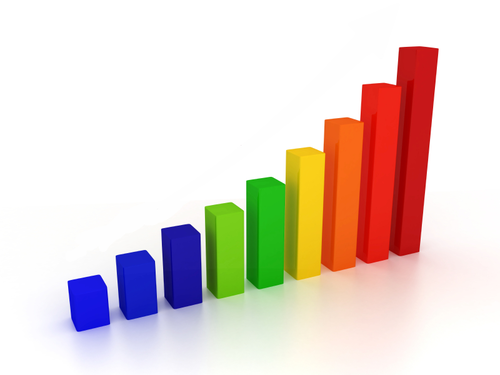
\includegraphics[width=0.5\textwidth]{graph.png}
  \caption{Графикон}
  \label{fig:grafikon}
\end{figure}

% primer jednostavnije matematičke formule
Ево и један пример математичке формуле: \(e^{i\pi} + 1 = 0\).
% naravno, dozvoljeno je koristiti i dobri stari $...$ stil, ali je \(...\) 
% više u duhu LaTeX-a i ima određene prednosti (npr. jasnije poruke o greškama)

% primer referisanja na sliku
На слици \ref{fig:grafikon} приказан је један графикон.

% primer kompleksnije matematičke formule
\[
\int_a^b f(x)\ \mathrm{d}x \ =_{def}\ \lim_{\max{\Delta x_k \rightarrow 0}} \sum_{k=1}^n f(x_k^*)\Delta x_k
\]
% slično kao i malo pre, dozvoljeno je koristiti i $$...$$, ali \[...\] ima
% određenih prednosti

% primer referisanja na poglavlja i strane poglavlja
Више детаља биће дато у глави \ref{chp:razrada} на страни \pageref{chp:razrada}.


% primer listinga koda

У тезу можемо убацити и програмски кôд.

\begin{verbatim}
Ovo je doslovni tekst.
\end{verbatim}

\begin{english}
\lstset{
language=C,
basicstyle=\ttfamily,
keywordstyle=\color{blue}
}
\begin{lstlisting}
#include <stdio.h>

int main() {
   printf("Hello, world!\n");
   return 0;
}
\end{lstlisting}
\end{english}


Овај C програм се може превести помоћу преводиоца GCC \cite{gcc}.

% primer liste
Можемо правити и набрајања:
\begin{enumerate}
\item Анализа 1
\item Линеарна алгебра
\item Аналитичка геометрија
\item Основи програмирања
\end{enumerate}

% primer nenumerisane liste
Набрајање може бити и ненумерисано:

\begin{itemize}
\item Анализа 1
\item Линеарна алгебра
\item Аналитичка геометрија
\item Основи програмирања
\end{itemize}

% primer opisne liste
Описне листе се користе када се описује свака од неколико ставки.

\begin{description}
\item[pdflatex] - класични преводилац за \LaTeX који користи специфичне фонтове.
\item[xelatex] - модернији преводилац за \LaTeX који користи
  \lat{OpenType} и \lat{TrueType} фонтове.
\end{description}

\pangrami

% ------------------------------------------------------------------------------
\chapter[Разрада]{Разрада - ово поглавље има страшно дугачак наслов који не може да стане само у један ред}
\label{chp:razrada}
% ------------------------------------------------------------------------------

\pangrami

\pangrami

% ------------------------------------------------------------------------------
\chapter{Закључак}
% ------------------------------------------------------------------------------
\pangrami

\pangrami

% ------------------------------------------------------------------------------
% Literatura
% ------------------------------------------------------------------------------
\literatura

% ==============================================================================
% Završni deo teze i prilozi
\backmatter
% ==============================================================================

% ------------------------------------------------------------------------------
% Biografija doktoranda
\begin{biografija}
\textbf{Вук Стефановић Караџић} (\emph{Тршић, 26. октобар/6. новембар
  1787. — Беч, 7. фебруар 1864.}) био је српски филолог, реформатор
српског језика, сакупљач народних умотворина и писац првог речника
српског језика.  Вук је најзначајнија личност српске књижевности прве
половине XIX века. Стекао је и неколико почасних доктората.
Учествовао је у Првом српском устанку као писар и чиновник у
Неготинској крајини, а након слома устанка преселио се у Беч,
1813. године. Ту је упознао Јернеја Копитара, цензора словенских
књига, на чији је подстицај кренуо у прикупљање српских народних
песама, реформу ћирилице и борбу за увођење народног језика у српску
књижевност. Вуковим реформама у српски језик је уведен фонетски
правопис, а српски језик је потиснуо славеносрпски језик који је у то
време био језик образованих људи. Тако се као најважније године Вукове
реформе истичу 1818., 1836., 1839., 1847. и 1852.
\end{biografija}
% ------------------------------------------------------------------------------


% Prilog 1: Izjava o autorstvu
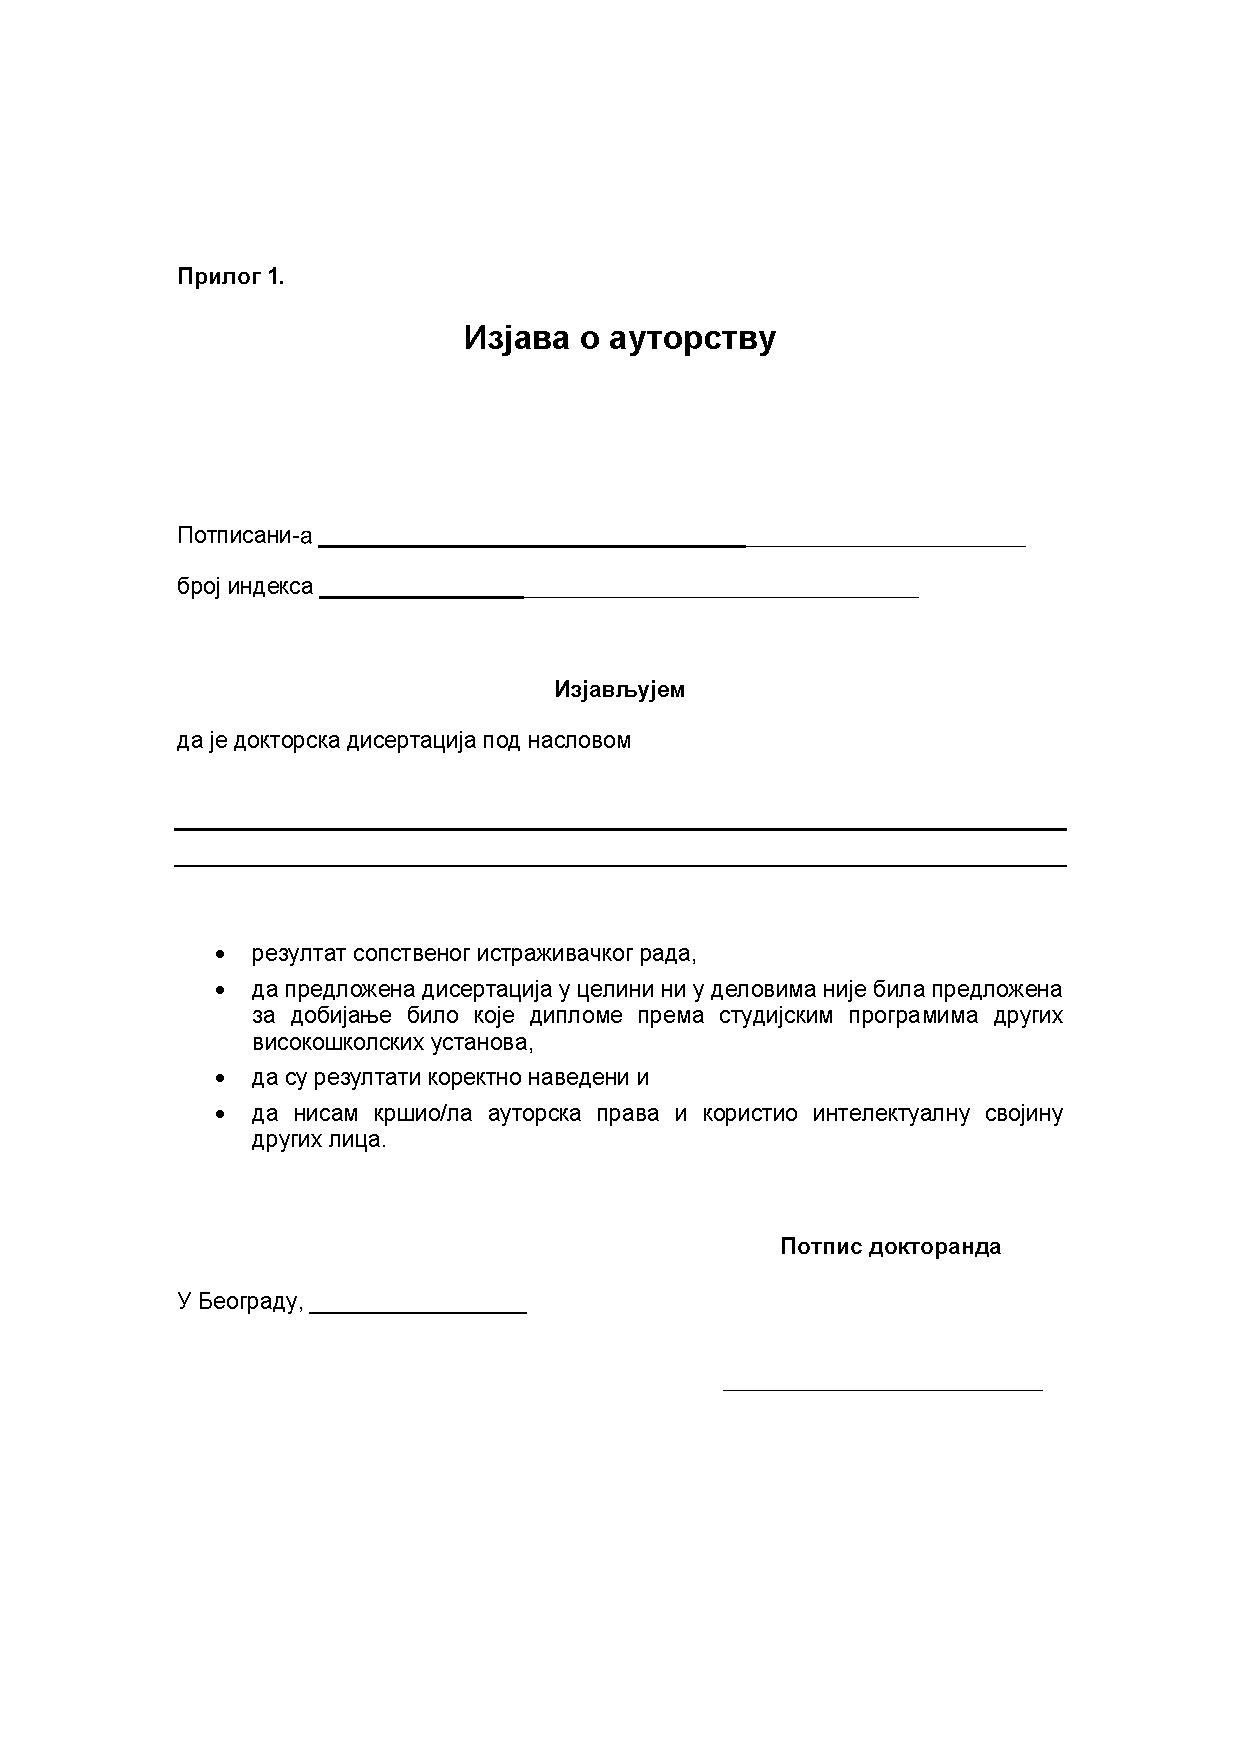
\includepdf{_Prilog1.pdf}
% Prilog 2: Izjava o istovetnosti štampane i elektronske verzije doktorskog rada
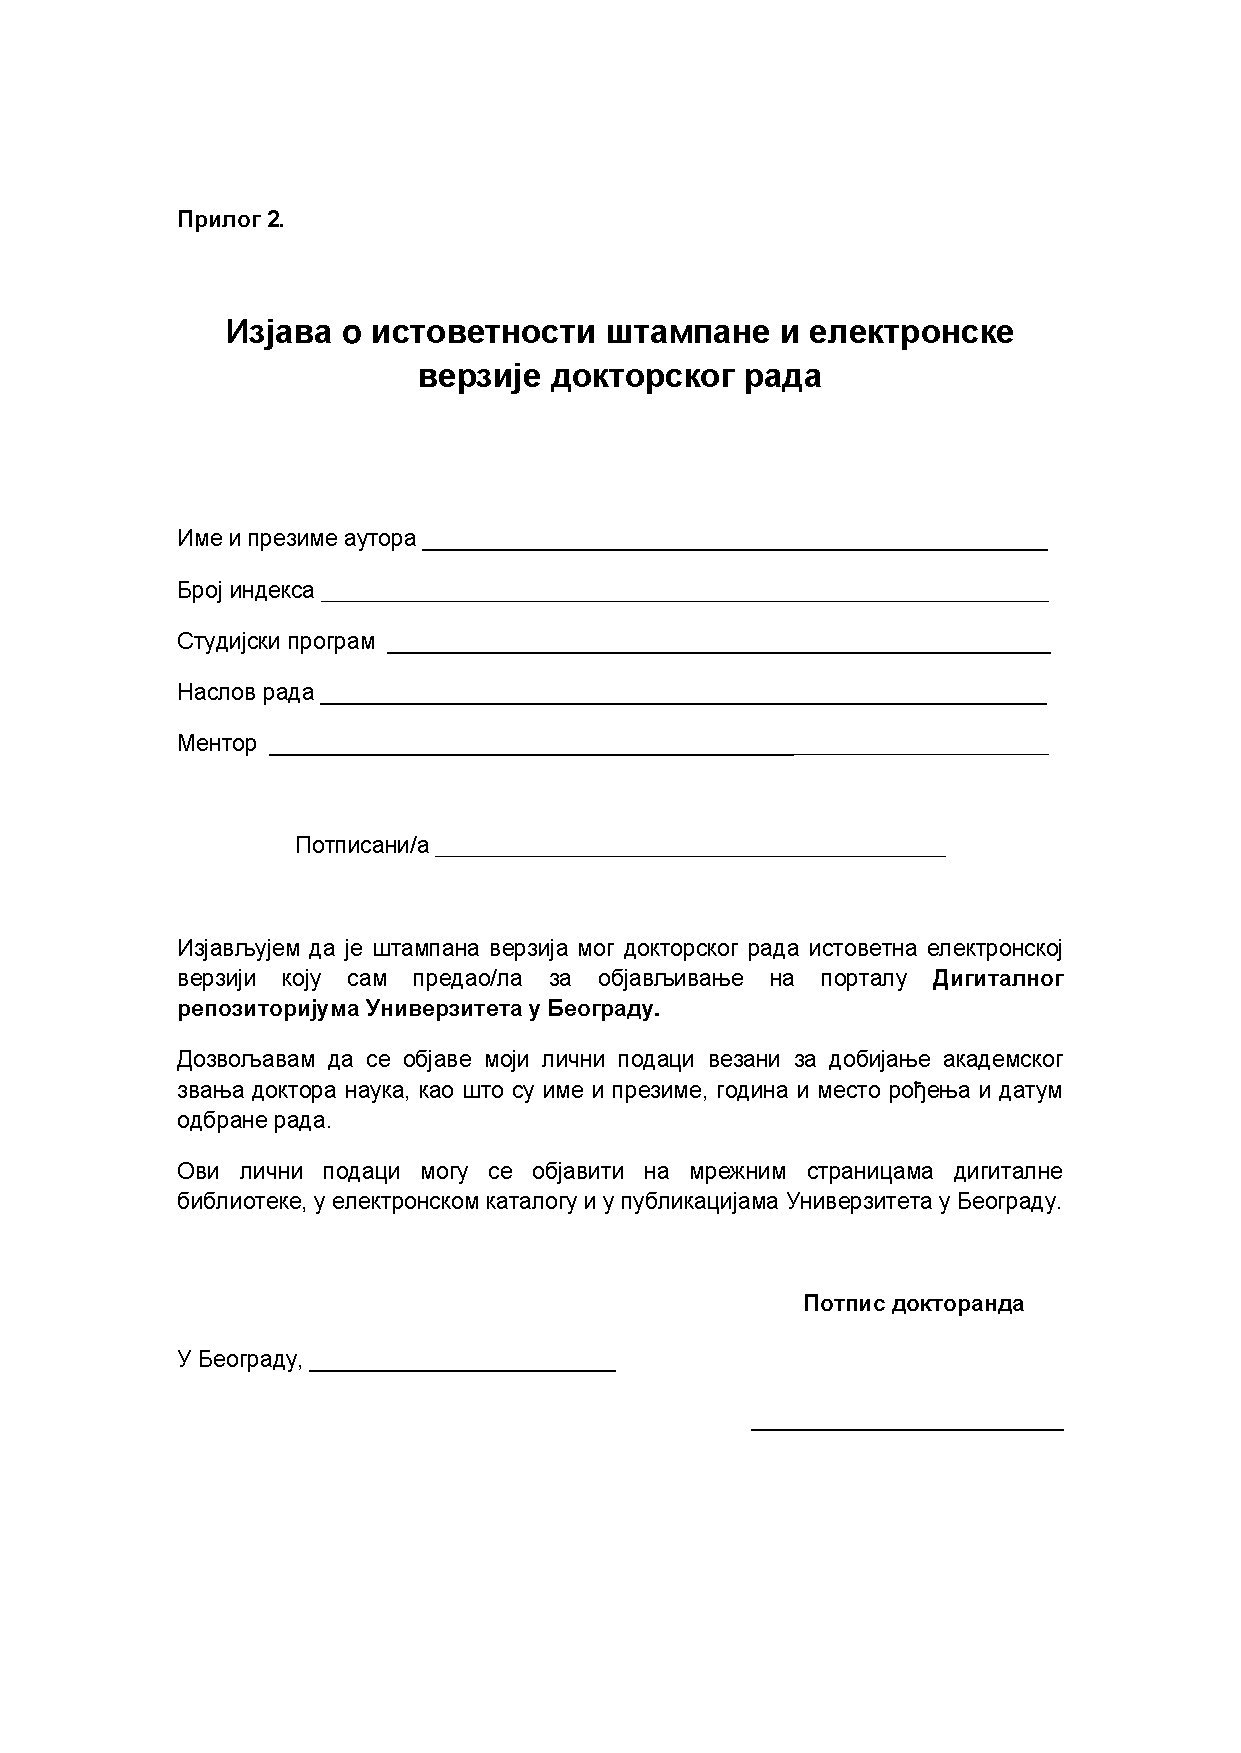
\includepdf{_Prilog2.pdf}
% Prilog 3: Izjava o korišćenju
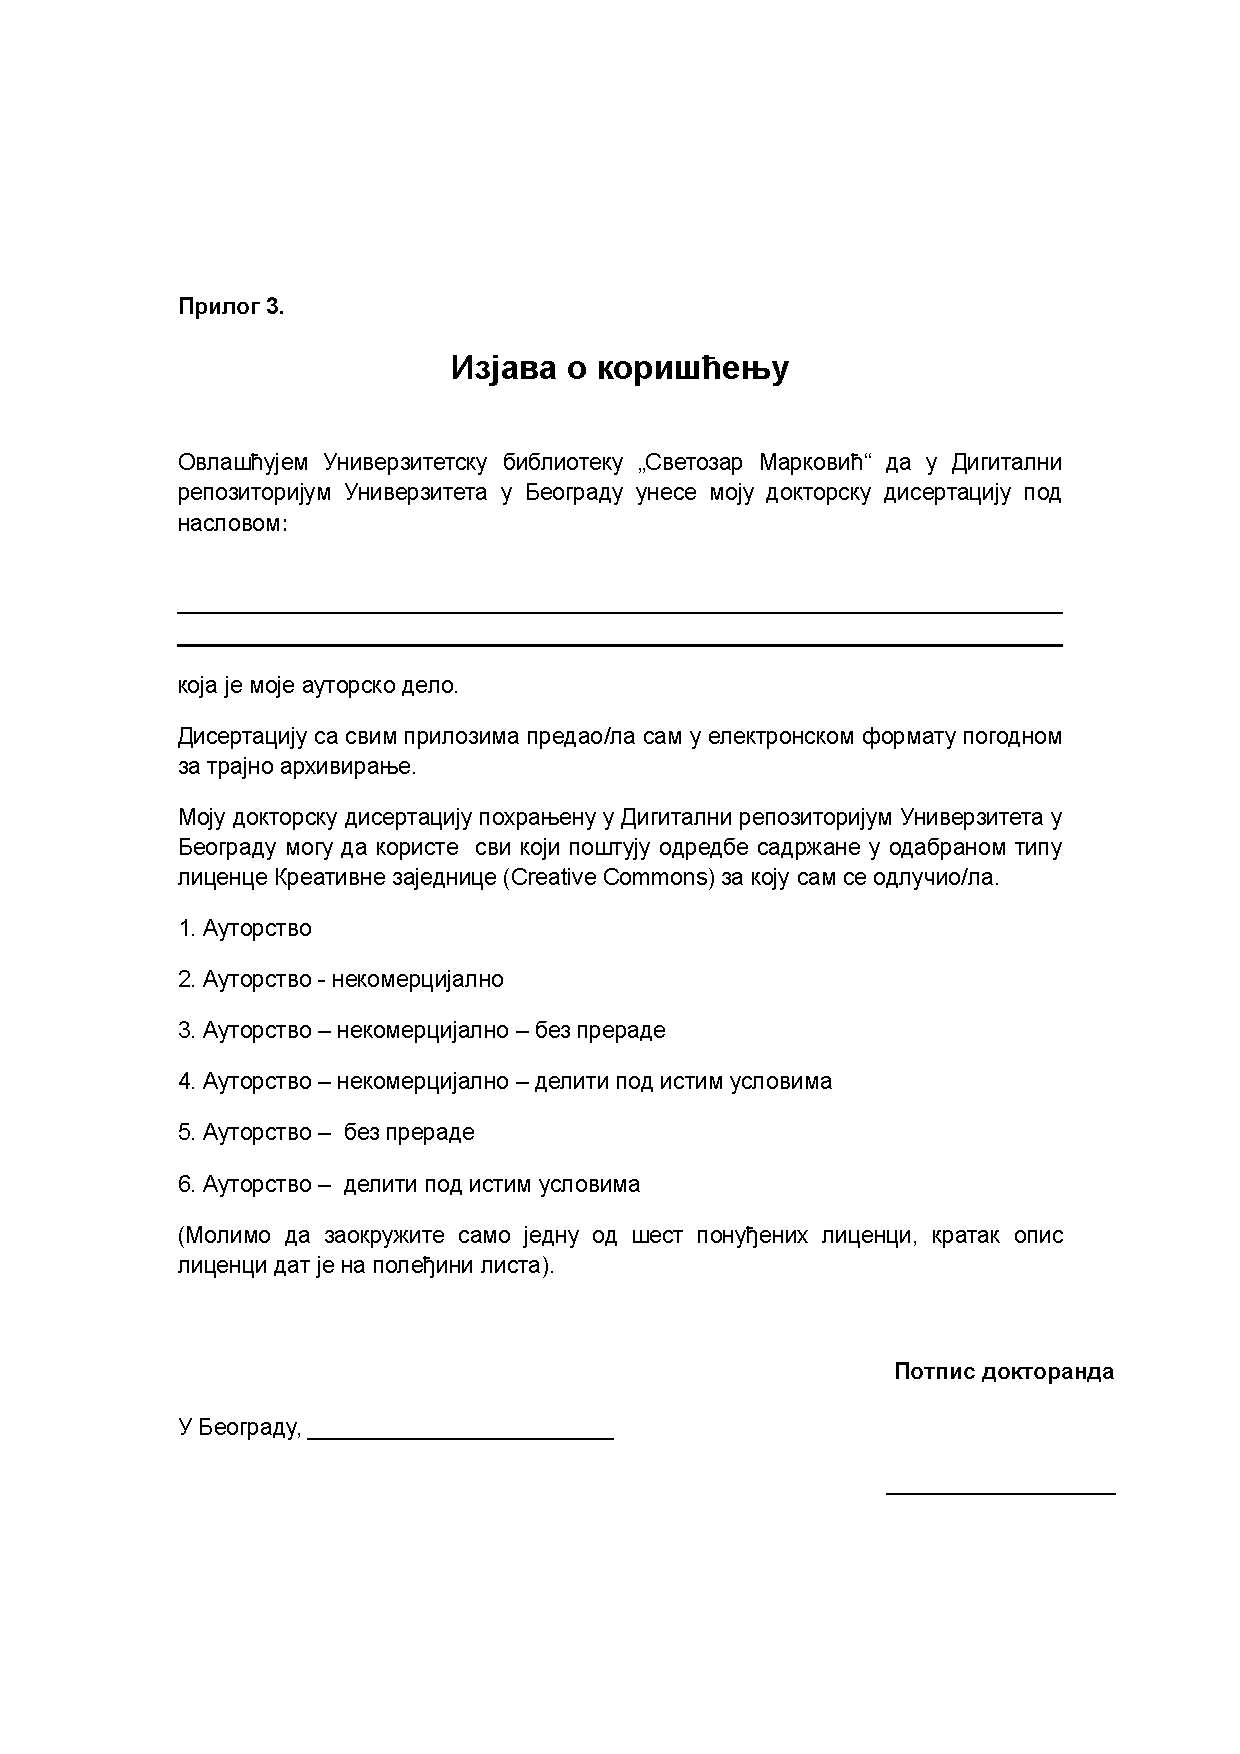
\includepdf{_Prilog3.pdf}

\end{document} 